\begin{figure}[H]
    \centering
    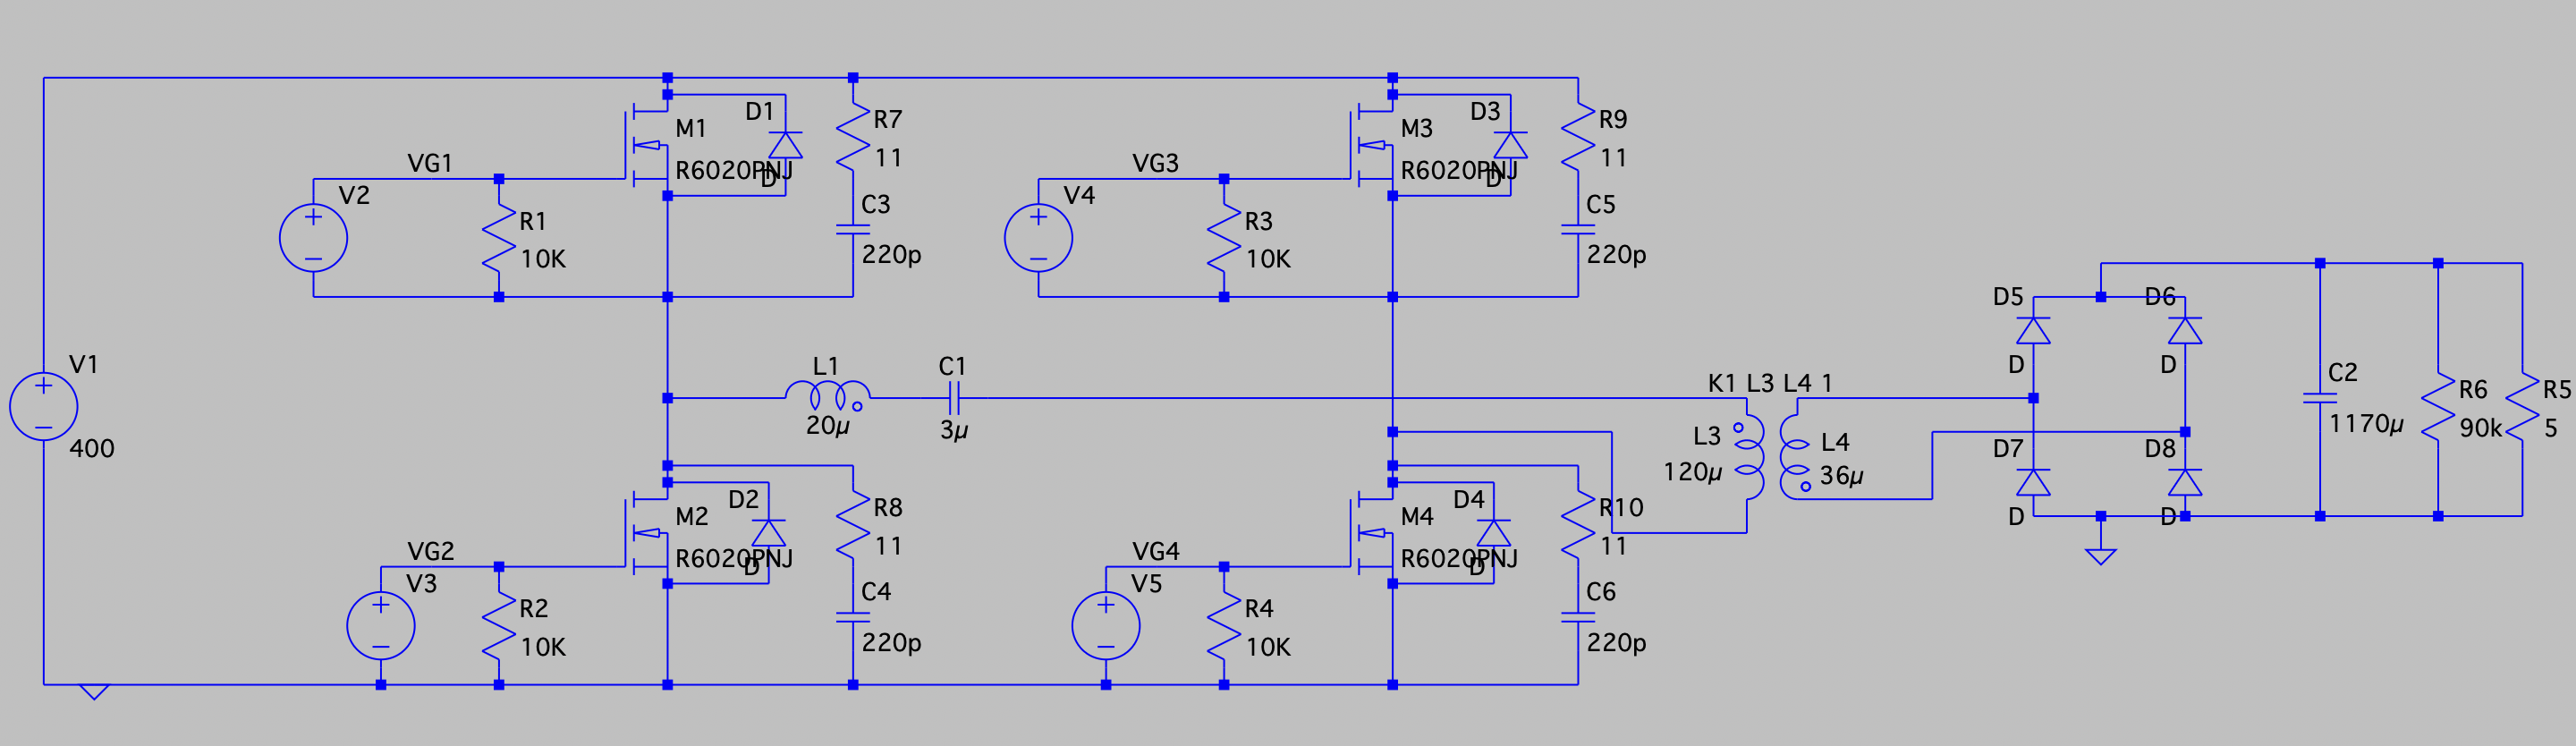
\includegraphics[width=\textwidth]{overall_circuit.png}
    \caption{Overall Circuit of the LLC Converter}
    \label{fig:Simulation1}
\end{figure}

\subsection{Sectional Analysis}
One of my first tasks was to perform a sectional analysis of the complete motherboard and control board circuit.
\noindent
Since active feedback is not possible in LtSpice, I decided to split the complete circuit into multiple sections, such as gate driver circuit, switching circuit, voltage feedback op-amps and circuit, etc. and then simulate them individually.\\
\begin{figure}[H]
    \centering
    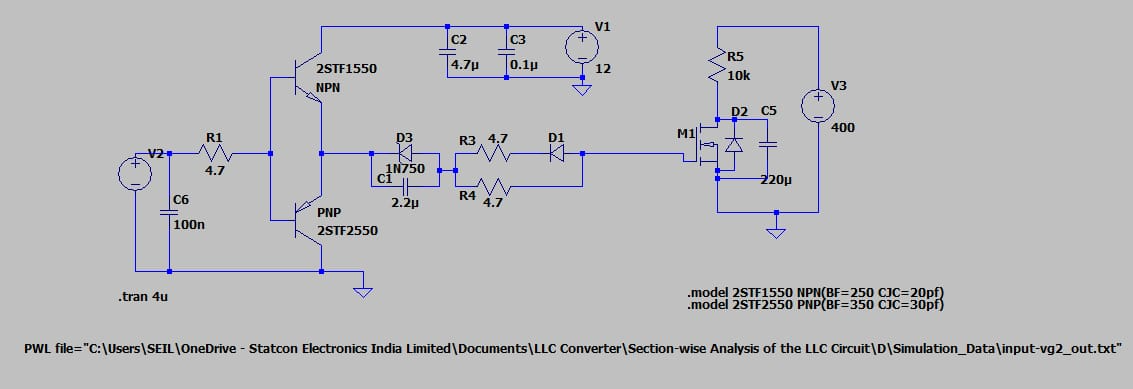
\includegraphics[width=\textwidth]{lt_circuit.png}
    \caption{LtSpice circuit of the gate driver circuit}
    \label{fig:lt_circuit}
\end{figure}

\noindent
One such circuit is shown in figure \ref*{fig:lt_circuit}
\noindent
The circuit shown above is of a gate driver circuit. This circuit is responsible for driving the MOSFETs in the switching circuit. The input to this circuit is a signal coming from the gate driver IC which in turn receives the signal generated by the microcontroller. The output of this circuit is the gate signal for the MOSFETs.\\

\subsection{Probing Actual Data}
To ensure that the hardware circuit is functioning as expected, data was probed using an oscilloscope with isolated probes (so as we do not to mess up the Gate signal of the MOSFETs while probing the data) as shown in figure \ref*{fig:oscilloscope_probe}
\begin{figure}[H]
    \centering
    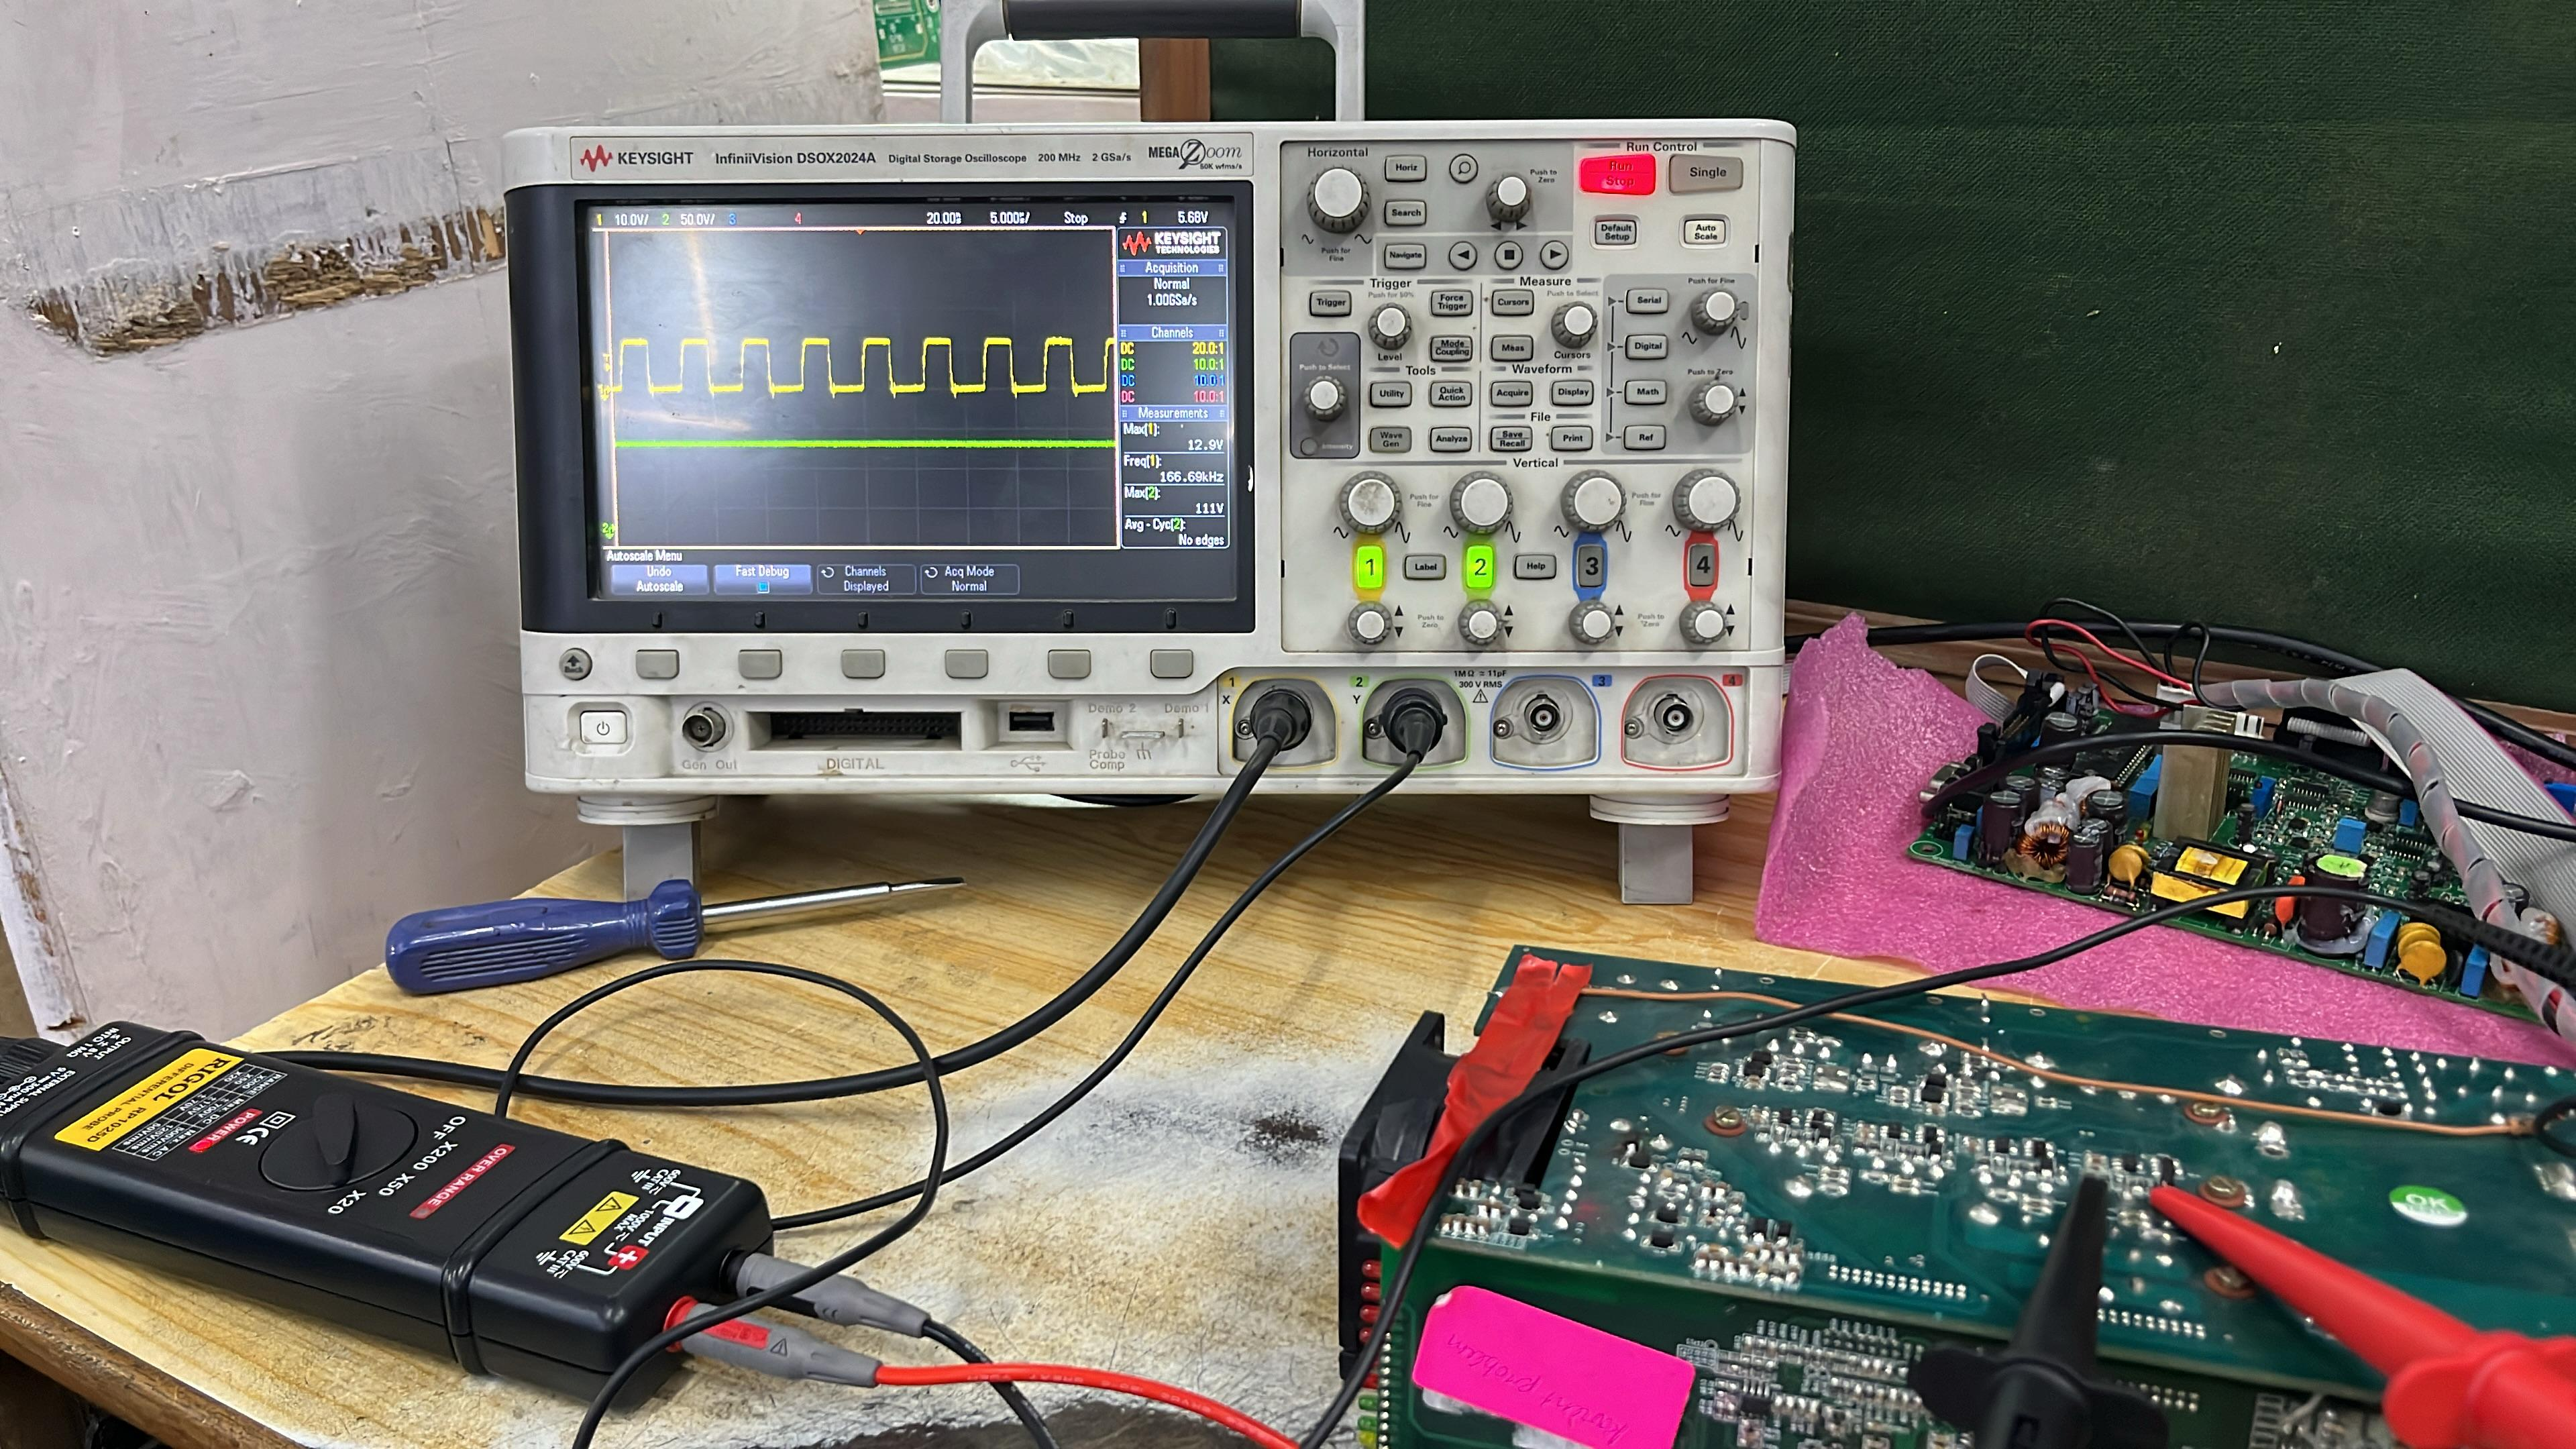
\includegraphics[width=\textwidth]{oscilloscope_probe1.jpg}
    \caption{Simulation}
    \label{fig:oscilloscope_probe}
\end{figure}

\subsection{Comparitive Analysis of Simulated Data with Actual Data}
The data obtained from the simulation was compared with the data obtained from the oscilloscope to ensure that the circuit is functioning as expected.
\noindent
This was done by writing a python script (.py file) which reads the data from the file generated by the oscilloscope as well as the file generated by LtSpice and then plots them on the same graph. (Figure \ref*{fig:sec_out})
\begin{figure}[H]
    \centering
    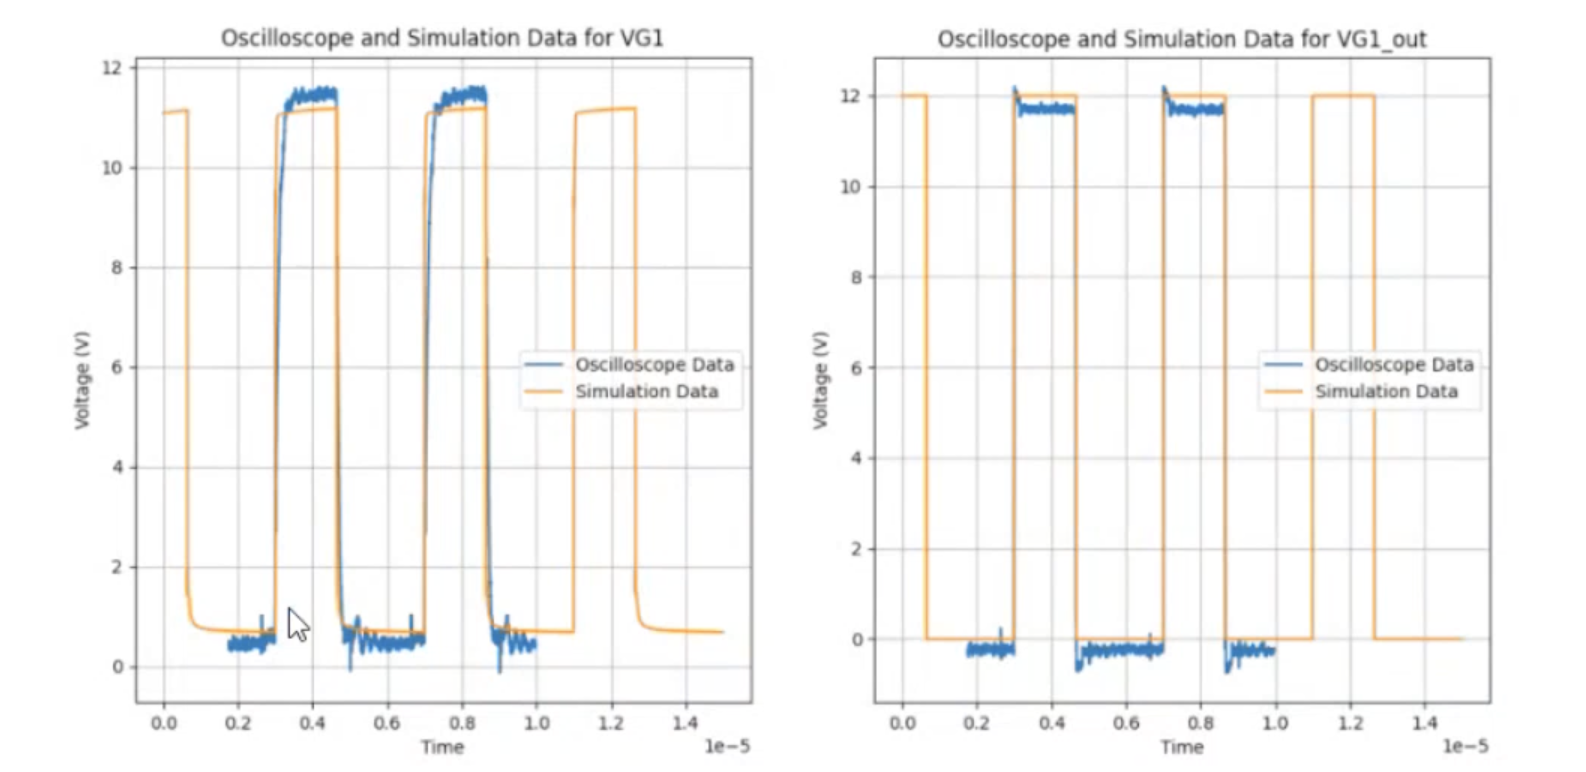
\includegraphics[width=\textwidth]{sectional_output.png}
    \caption{Comparision of Simulated and Probed Data for 2 signals}
    \label{fig:sec_out}
\end{figure}